\begin{figure}[H]
\centering
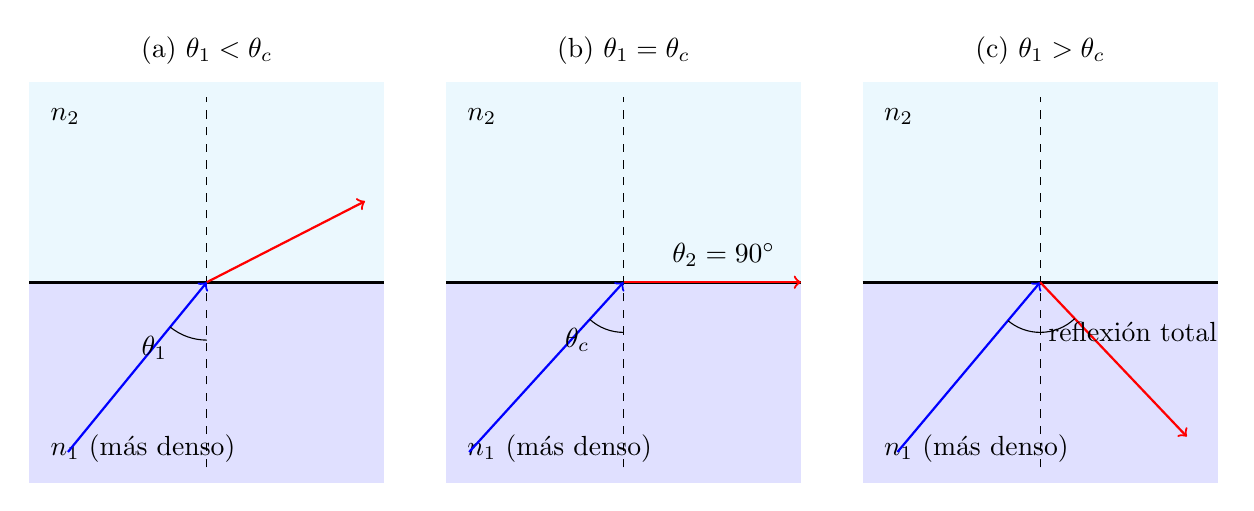
\begin{tikzpicture}[scale=0.98]
  \foreach \s in {0,5.4,10.8}{
    \fill[cyan!8] (\s,0) rectangle +(4.6,2.6);
    \fill[blue!12] (\s,-2.6) rectangle +(4.6,2.6);
    \draw[very thick] (\s,0) -- +(4.6,0);
    \draw[dashed] (\s+2.3,-2.4) -- +(0,4.8);
    \node[anchor=west] at (\s+0.15,2.15) {$n_2$};
    \node[anchor=west] at (\s+0.15,-2.15) {$n_1$ (más denso)};
  }
  \node at (2.3,3.0) {(a) $\theta_1<\theta_c$};
  \node at (7.7,3.0) {(b) $\theta_1=\theta_c$};
  \node at (13.1,3.0) {(c) $\theta_1>\theta_c$};
  \draw[->,blue,thick] (0.5,-2.2) -- (2.3,0);
  \draw[->,red,thick] (2.3,0) -- (4.35,1.05);
  \draw (2.3,-0.75) arc[start angle=-90,end angle=-129.4,radius=0.75];
  \node at (1.62,-0.85) {$\theta_1$};
  \draw[->,blue,thick] (5.7,-2.2) -- (7.7,0);
  \draw[->,red,thick] (7.7,0) -- (10.0,0);
  \draw (7.7,-0.65) arc[start angle=-90,end angle=-132.3,radius=0.65];
  \node at (7.1,-0.75) {$\theta_c$};
  \node at (9.0,0.35) {$\theta_2=90^\circ$};
  \draw[->,blue,thick] (11.25,-2.2) -- (13.1,0);
  \draw[->,red,thick] (13.1,0) -- (15.0,-2.0);
  \draw (13.1,-0.65) arc[start angle=-90,end angle=-130,radius=0.65];
  \draw (13.1,-0.65) arc[start angle=-90,end angle=-46.5,radius=0.65];
  \node at (14.3,-0.65) {reflexión total};
\end{tikzpicture}
\caption{Refracción, ángulo crítico y reflexión interna total.}
\end{figure}